\documentclass[10pt,a4paper]{article}
\usepackage{amsmath}
\usepackage{amssymb}
\usepackage{graphicx}
\usepackage{color}
\usepackage{fancyhdr}
\usepackage{fancyvrb}
\usepackage[margin=3.5cm]{geometry}
\usepackage{framed}
\usepackage{enumerate}
\usepackage{textcomp}
\def\ket#1{\left|#1\right\rangle}
\def\bra#1{\left\langle#1\right|}
\def\braket#1{\left\langle#1\right\rangle}

\definecolor{linkcol}{rgb}{0.0, 0.0, 0.7}
\usepackage[colorlinks=true,urlcolor=linkcol,citecolor=black,linkcolor=linkcol]{hyperref}

\setcounter{section}{8}
\renewcommand\thesection{\arabic{section}}
\renewcommand\thesubsection{\thesection.\arabic{subsection}}

\fancyhf{}
\lhead{\tiny Y.~D.~Chong (2020)}
\rhead{\scriptsize MH2801: Complex Methods for the Sciences}
\lfoot{}
\rfoot{\thepage}
\pagestyle{fancy}

\begin{document}
\setcounter{page}{73}

\section{Fourier Series and Fourier Transforms}
\label{fourier-series-and-fourier-transforms}

The \textbf{Fourier transform} is one of the most important mathematical
tools used for analyzing functions. The basic idea is that an arbitrary
function $f(x)$, with a real domain ($x \in \mathbb{R}$), can be
expressed as a linear combination of more elementary functions
(sinusoidal waves). The coefficients of this linear combination form a
counterpart function, $F(k)$, that is defined in a wave-number domain
($k \in \mathbb{R}$). As it turns out, it's often more convenient to
deal with $F(k)$, because certain mathematical problems, such as
differential equations, are easier to solve in the wave-number domain.

\subsection{Fourier series}\label{fourier-series}

We begin by discussing the \textbf{Fourier series}, which is used to
analyze functions which are periodic in their inputs. A \textbf{periodic
function} $f(x)$ is a function of a real variable $x$ that repeats
itself every time $x$ changes by $a$, as shown in the figure below:

\begin{figure}[h]
  \centering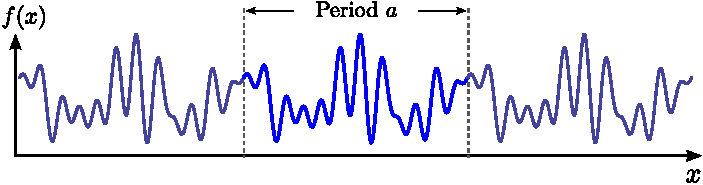
\includegraphics[width=0.6\textwidth]{periodicity}
\end{figure}

The constant $a$ is called the \textbf{period}. We can write the
periodicity condition as
\begin{equation}
f(x+a) = f(x), \;\; \forall\; x\in \mathbb{R}.
\end{equation}
The value of $f(x)$ can be real or complex, but $x$ should be real.
Another equivalent way to think of a periodic function is as a function
defined over a finite domain $-a/2 \le x < a/2$, with periodic
boundary conditions $f(-a/2) = f(a/2)$.

You can think of $x$ as representing a spatial coordinate. (The
following mathematical discussion also applies to functions of time,
with minor differences in convention that we will discuss in Section
\ref{fourier-transforms-for-time-domain-functions}.)

Let's consider what it means to ``specify'' a periodic function
$f(x)$. One way to specify the function is to give an explicit
mathematical formula for it, but not all functions can be described by a
formula. Another approach might be to specify the function values in
$-a/2 \le x < a/2$. Since there's an uncountably infinite number of
points in this domain, we can generally only achieve an
\emph{approximate} specification of $f$ this way. This is done by
specifying the values of $f(x)$ for a large (but finite) set of $x$
points.

There is another method for specifying $f$ that is perhaps less
obvious. We could express the function as a linear combination of
simpler periodic functions, consisting of sines and cosines:
\begin{equation}
f(x) = \sum_{n=1}^\infty \alpha_n \sin\left(\frac{2\pi n x}{a}\right) + \sum_{m=0}^\infty \beta_m \cos\left(\frac{2 \pi m x}{a}\right).
\end{equation}
This is called a \textbf{Fourier series}. If the set of numbers
$\{\alpha_n, \beta_m\}$, which are called the \textbf{Fourier
coefficients}, are specified, then $f(x)$ can be calculated for any
$x$. Note that the Fourier coefficients are real if $f(x)$ is a real
function, or complex if $f(x)$ is complex.

The justification for the Fourier series formula is that the sine and
cosine functions in the series are, themselves, periodic with period
$a$:
\begin{align}
  \sin\left(\frac{2\pi n (x+a)}{a}\right) = \sin\left(\frac{2\pi n x}{a} + 2\pi n\right) &= \sin\left(\frac{2\pi n x}{a}\right)\\ \cos\left(\frac{2\pi m (x+a)}{a}\right) = \cos\left(\frac{2\pi m x}{a} + 2\pi m\right) &= \cos\left(\frac{2\pi m x}{a}\right)
\end{align}
Hence, any such linear combination automatically satisfies the
periodicity condition for $f$. (Note that in the Fourier series
formula, the sum over $n$ starts from 1, but the sum over $m$ starts
from 0. This is because the sine term with $n = 0$ is zero for all
$x$, so it's redundant.)

\subsubsection{Square-integrable functions}
\label{square-integrable-functions}

If a periodic function is expressible as a Fourier series, the Fourier
coefficients seem like a nice way of describing it. But can arbitrary
periodic functions always be expressed as a Fourier series? This
question turns out to be surprisingly intricate, and its resolution
preoccupied mathematicians for much of the 19th century;
\href{http://en.wikipedia.org/wiki/Convergence_of_Fourier_series}{the
full answer} is beyond the scope of our present discussion.

Luckily, it turns out that a certain class of periodic functions, which
are commonly encountered in physical contexts, are guaranteed to
\emph{always} be expressible as Fourier series. These are called
\textbf{square-integrable functions}, defined as functions for which the
integral
\begin{equation}
\int_{-a/2}^{a/2} dx\; \big|\,f(x)\,\big|^2
\end{equation}
exists and is finite. Unless otherwise stated, we will always assume
that the functions we're dealing with are square-integrable.

\subsubsection{Complex Fourier series and inverse relations}
\label{complex-fourier-series-and-inverse-relations}

Using Euler's formula, we can re-write the Fourier series as follows:
\begin{equation}
f(x) = \sum_{n=-\infty}^\infty e^{2\pi i n x/a}\, f_n.
\end{equation}
Instead of separate sums over sines and cosines, we have a single sum
over complex exponentials, which is neater. The sum includes negative
integers $n$, and involves a new set of Fourier coefficients, $f_n$,
which are complex numbers. (As an exercise, try working out how the
old coefficients $\{\alpha_n, \beta_n\}$ are related to the new
coefficients $\{f_n\}$.)

If the Fourier coefficients $\{f_n\}$ are known, then $f(x)$ can be
calculated using the above formula. The converse is also true: given
$f(x)$, we can determine the Fourier coefficients. To see how, observe
that
\begin{equation}
\int_{-a/2}^{a/2} dx \; e^{-2\pi i m x/a}\, e^{2\pi i n x/a} = a\, \delta_{mn}\quad \mathrm{for}\;m, n \in \mathbb{Z},
\end{equation}
where $\delta_{mn}$ is the
\href{http://en.wikipedia.org/wiki/Kronecker_delta}{Kronecker delta},
defined as:
\begin{equation}
\delta_{mn} = \left\{\begin{array}{ll}1, & \textrm{if}\; m = n\\ 0, & \mathrm{if}\;m\ne n.\end{array}\right.
\end{equation}
Due to this property, the set of functions $\exp(2\pi i n x / a)$,
with integer values of $n$, are said to be \textbf{orthogonal}
functions. (We won't go into the details now, but the term
``orthogonality'' is used here with the same meaning as in vector
algebra, where a set of vectors $\vec{v}_1, \vec{v}_2, \dots$ is said
to be ``orthogonal'' if $\vec{v}_m \cdot \vec{v}_n = 0$ for
$m\ne n$.) Hence,
\begin{align}
  \int_{-a/2}^{\,a/2} dx\; e^{-2\pi i m x/a} \;f(x)
  &= \, \int_{-a/2}^{\,a/2} dx\; e^{-2\pi i m x/a} \left[\sum_{n=-\infty}^\infty e^{2\pi i n x/a}\, f_n\right] \\
  &= \sum_{n=-\infty}^\infty \, \int_{-a/2}^{\,a/2} dx\; e^{-2\pi i m x/a}  \, e^{2\pi i n x/a} \;f_n \\
  &= \sum_{n=-\infty}^\infty \, a\, \delta_{mn} \, f_n \\
  &= a \,f_m.
\end{align}
The procedure of multiplying by $\exp(-2\pi i m x/a)$ and integrating
over $x$ acts as a kind of ``sieve'', filtering out all other Fourier
components of $f(x)$ and keeping only the one with the matching index
$m$. Thus, we arrive at a pair of relations expressing $f(x)$ in
terms of its Fourier components, and vice versa:

\begin{framed} \noindent
  \begin{align}
    \begin{aligned}
      \left\{\;\;\begin{array}{rl}f(x) &= \displaystyle \, \sum_{n=-\infty}^\infty e^{i k_n x}\, f_n \\ f_n &= \displaystyle\,\frac{1}{a} \int_{-a/2}^{\,a/2} dx\; e^{-i k_n x}\, f(x)\end{array}\;\;\right. \quad\quad\mathrm{where}\;\; k_n \equiv \frac{2\pi n}{a}
      \label{fseries}
    \end{aligned}
  \end{align}
\end{framed}

The real numbers $k_n$ are called \textbf{wave-numbers}. They form a
discrete set, with one for each Fourier component. In physics jargon, we
say that the wave-numbers are ``quantized'' to integer multiples of
$\Delta k \equiv 2\pi/a.$

\subsubsection{Example: Fourier series of a square wave}
\label{example-fourier-series-of-a-square-wave}

To get a feel for how the Fourier series behaves, let's look at a square
wave: a function that takes only two values $+1$ or $-1$, jumping
between the two values at periodic intervals. Within one period, the
function is
\begin{equation}
f(x) = \left\{\begin{array}{ll}-1, & -a/2 \le x < 0 \\ +1, & \quad\;\;\; 0 \le x < a/2.\end{array}\right.
\end{equation}
Plugging this into the Fourier relation, and doing the straightforward
integrals, gives the Fourier coefficients
\begin{equation}
\begin{aligned} f_n &= -i \, \frac{\left[\sin\left(n \pi/2\right)\right]^2}{n\pi/2 } \\ &= \left\{\begin{array}{cl} -2i/n\pi ,& n \; \mathrm{odd} \\ 0,& n \; \mathrm{even}. \\\end{array}\right.\end{aligned}
\end{equation}
As can be seen, the Fourier coefficients become small for large $n$.
We can write the Fourier series as
\begin{equation}
f(x) \; \leftrightarrow \; \sum_{n=1,3,5,\dots} \frac{4\sin(2\pi n x / a)}{n \pi}.
\end{equation}
If this infinite series is truncated to a finite number of terms, we get
an approximation to $f(x)$. In the
following figure, we show the Fourier series truncated up to $N
= 5$ and $N= 29$:

\begin{center}
  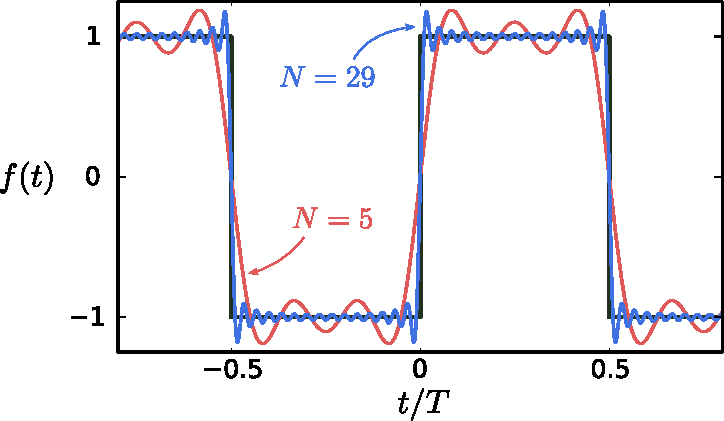
\includegraphics[width=0.6\textwidth]{square_fourier}
\end{center}

One amusing (but apparently useless) consequence of the above result is
that we can use it to derive a series expansion for $\pi$. If we set
$x = a/4$,
\begin{equation}
f(a/4) = 1 = \frac{4}{\pi} \left[\sin(\pi/2) + \frac{1}{3}\sin(3\pi/2) + \frac{1}{5}\sin(5\pi/2) + \cdots\right],
\end{equation}
and hence
\begin{equation}
\pi = 4 \left(1 - \frac{1}{3} + \frac{1}{5} - \frac{1}{7} + \cdots\right).
\end{equation}

\subsection{Fourier transforms}
\label{fourier-transforms}

The Fourier series applies to periodic functions defined over the
interval $-a/2 \le x < a/2$.  But the concept can be generalized to
functions defined over the entire real line, $x \in \mathbb{R}$, if we
take the limit $a \rightarrow \infty$ carefully.

Suppose we have a function $f$ defined over the entire real line, $x
\in \mathbb{R}$, such that $f(x) \rightarrow 0$ for $x \rightarrow
\pm\infty$. Imagine there is a family of periodic functions
$\big\{f_a(x) \,\big|\, a \in\mathbb{R}^+\big\}$, such that $f_a(x)$
has periodicity $a$, and approaches $f(x)$ in the limit $a\rightarrow
\infty$. This is illustrated in the figure below:

\begin{center}
  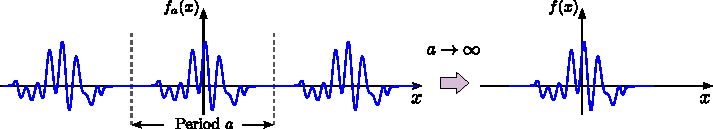
\includegraphics[width=0.99\textwidth]{periodicity_ft}
\end{center}

In mathematical terms,
\begin{equation}
f(x) = \lim_{a \rightarrow \infty} f_a(x), \;\;\;\text{where}\;\; f_a(x+a) = f_a(x).
\end{equation}
Since $f_a$ is periodic, it can be expanded as a Fourier series:
\begin{equation}
f_a(x) = \sum_{n=-\infty}^\infty e^{i k_n x}\, f_{an}, \quad\mathrm{where}\;\; k_n = n\Delta k, \;\; \Delta k = \frac{2\pi}{a}.
\end{equation}
Here, $f_{an}$ denotes the $n$-th complex Fourier coefficient of the
function $f_a(x)$. Note that each Fourier coefficient depends
implicitly on the periodicity $a$.

As $a \rightarrow \infty$, the wave-number quantum $\Delta k$ goes to
zero, and the set of discrete $k_n$ turns into a continuum. During
this process, each individual Fourier coefficient $f_{an}$ goes to
zero, because there are more and more Fourier components in the
vicinity of each $k$ value, and each Fourier component contributes
less. This implies that we can replace the discrete sum with an
integral over the values of $k_n$. To accomplish this, we first
multiply the summand by a factor of $(\Delta k/2\pi) / (\Delta k/2\pi)
= 1$:
\begin{equation}
f(x) = \lim_{a\rightarrow \infty} \left[\;\,\sum_{n=-\infty}^\infty \frac{\Delta k}{2\pi} \, e^{i k_n x}\, \left(\frac{2\pi \,f_{an}}{\Delta k} \right)\;\,\right].
\end{equation}
(In case you're wondering, the choice of $2\pi$ factors is essentially
arbitrary; we are following the usual convention.) Moreover, we define
\begin{equation}
F(k) \equiv \lim_{a \rightarrow \infty} \left[\frac{2\pi\, f_{an}}{\Delta k}\right]_{k = k_n}.
\end{equation}
In the $a \rightarrow \infty$ limit, the $f_{an}$ in the numerator
and the $\Delta k$ in the denominator both go zero, but if their ratio
remains finite, we can turn the Fourier sum into the following integral:
\begin{equation}
f(x) = \int_{-\infty}^{\infty} \frac{dk}{2\pi} \, e^{i k x}\, F(k).
\end{equation}

\subsubsection{The Fourier relations}\label{the-fourier-relations}

The function $F(k)$ defined in the previous section is called the
\textbf{Fourier transform} of $f(x)$. Just as we have expressed $f(x)$
in terms of $F(k)$, we can also express $F(k)$ in terms of $f(x)$. To
do this, we apply the $a \rightarrow \infty$ limit to the second
equation in \eqref{fseries}:
\begin{align}
  F(k_n) &= \lim_{a\rightarrow \infty} \frac{2 \pi\, f_{an}}{\Delta k} \\
 &= \lim_{a\rightarrow \infty} \frac{2 \pi}{2\pi/a}\, \left(\frac{1}{a} \int_{-a/2}^{a/2} dx\; e^{-i k_n x}\right) \\
  &= \int_{-\infty}^\infty dx\; e^{-i kx}\, f(x).
\end{align}
Hence, we arrive at a pair of equations called the \textbf{Fourier
relations}:

\begin{framed}
  \begin{align}
    F(k) &= \;\int_{-\infty}^\infty dx\; e^{-ikx}\, f(x) \label{ft}\\
    f(x) &= \int_{-\infty}^\infty \frac{dk}{2\pi}\; e^{ikx}\, F(k) \label{ift}
  \end{align}
\end{framed}

\noindent
Eq.~\eqref{ft} is called the Fourier transform, and Eq.~\eqref{ift} is
called the \textbf{inverse Fourier transform}. These relations state
that if we have a function $f(x)$ defined over $x \in \mathbb{R}$,
then there is a unique counterpart function $F(k)$ defined over $k \in
\mathbb{R}$, and vice versa.

There are some differences between the two formulas. Firstly, there is
a factor of $1/2\pi$ appears next to $dk$, but no such factor for
$dx$; this is a matter of convention, tied to our earlier definition
of $F(k)$. Secondly, the integral over $x$ contains a factor of
$e^{-ikx}$ but the integral over $k$ contains a factor of
$e^{ikx}$. One way to remember which equation has the positive sign in
the exponent is to interpret the inverse Fourier transform equation
(which has the form of an integral over $k$) as the continuum limit of
a sum over complex waves. In this sum, $F(k)$ plays the role of the
series coefficients, and by convention the complex waves in the sum
have the form $\exp(ikx)$.

In our definition of the Fourier transform, it is clear that the
Fourier series needs to remain convergent as we take the $a
\rightarrow \infty$ limit. Based on the discussion of
Section~\ref{square-integrable-functions}, this means we are always
dealing with functions such that
\begin{equation}
\int_{-\infty}^{\infty} dx\; \big|\,f(x)\,\big|^2
\end{equation}
exists and is finite.

\subsubsection{A simple example}\label{a-simple-example}

Consider the function
\begin{equation}
f(x) = \left\{\begin{array}{cl}e^{-\eta x}, & x \ge 0 \\ 0, & x < 0,\end{array}\right. \qquad \eta \in \mathbb{R}^+.
\end{equation}
For $x < 0$, this is an exponentially-decaying function, and for
$x < 0$ it is identically zero. The real parameter $\eta$ is called
the decay constant; for $\eta > 0$, the function $f(x)$ vanishes as
$x \rightarrow +\infty$ and can thus be shown to be square-integrable,
and larger values of $\eta$ correspond to faster exponential decay.

The Fourier transform can be found by directly calculating the Fourier
integral:
\begin{equation}
F(k) \;=\; \;\int_{0}^\infty dx\; e^{-i kx}\, e^{-\kappa x} \;=\; \frac{-i}{k - i \eta}.
\end{equation}
It is useful to plot the squared magnitude of the Fourier transform,
$|F(k)|^2$, against $k$. This is called the \textbf{Fourier
spectrum} of $f(x)$. In this case,
\begin{equation}
\big|\,F(k)\,\big|^2 = \frac{1}{k^2 + \eta^2}.
\end{equation}
This Fourier spectrum is plotted in the figure below. It consists of a
peak centered at $k = 0$, forming a type of curve called a
\textbf{Lorentzian}. The width of the Lorentzian is dependent on the
original function's decay constant $\eta$. For small $\eta$,
i.e.~weakly-decaying $f(x)$, the peak is narrow; for large $\eta$,
i.e.~rapidly-decaying $f(x)$, the peak is broad.

\begin{figure}[h]
  \centering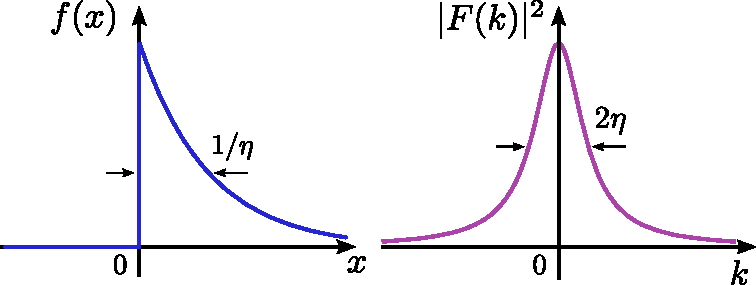
\includegraphics[width=0.7\textwidth]{fourier_example1}
\end{figure}

We can quantify the width of the Lorentzian by defining the
\textbf{full-width at half-maximum} (FWHM)---the width of the curve at
half the value of its maximum. In this case, the maximum of the
Lorentzian curve occurs at $k=0$ and has the value of $1/\eta^2$.  The
half-maximum, $1/2\eta^2$, occurs when $\delta k = \pm \eta$.  Hence,
the original function's decay constant, $\eta$, is directly
proportional to the FWHM of the Fourier spectrum, which is $2\eta$.

To wrap up this example, let's evaluate the inverse Fourier transform:
\begin{equation}
f(x) \; = \; -i\int_{-\infty}^\infty \frac{dk}{2\pi} \; \frac{e^{i kx}}{k-i\eta}.
\end{equation}
This can be done by contour integration. The analytic continuation of
the integrand has one simple pole, at $k = i\eta$. For $x < 0$, the
numerator $\exp(ikx)$ vanishes far from the origin in the lower
half-plane, so we close the contour below. This encloses no pole, so
the integral is zero. For $x > 0$, the numerator vanishes far from the
origin in the upper half-plane, so we close the contour above, with a
counter-clockwise arc.  Hence,
\begin{equation}
f(x) = \left(\frac{-i}{2\pi}\right) \, \left(2\pi i\right) \, \mathrm{Res}\left[ \frac{e^{ikx}}{k-i\eta}\right]_{k=i\eta} = e^{-\eta x} \qquad(x > 0)
\end{equation}
which is indeed the function that we started out with.

\subsection{Fourier transforms for time-domain functions}
\label{fourier-transforms-for-time-domain-functions}

So far, we have been dealing with functions of a spatial coordinate
$x$. Of course, mathematical relations don't care about what kind of
physical variable we are dealing with, so the same equations could be
applied to functions of time $t$. However, there is a important
difference in \emph{convention}. When dealing with functions of the time
coordinate $t$, it is customary to use a different sign convention in
the Fourier relations!

The Fourier relations for a function of time, $f(t)$, are:
\begin{framed}
  \begin{align}
    F(\omega) &= \;\int_{-\infty}^\infty dt\; e^{i\omega t}\, f(t) \\ f(t) &= \int_{-\infty}^\infty \frac{d\omega}{2\pi}\; e^{-i\omega t}\, F(\omega).
  \end{align}
\end{framed}

\noindent
Compared to Eqs.~\eqref{ft} and \eqref{ift}, the signs of the $\pm i
\omega t$ exponents are flipped.

There's a good reason for this difference in sign convention: it
arises from the need to describe propagating waves, which vary with
both space \emph{and} time. As we have previously discussed, a
propagating plane wave can be described by a wavefunction of the form
\begin{equation}
f(x,t) = A e^{i(kx - \omega t)},
\end{equation}
where $k$ is the wave-number and $\omega$ is the angular frequency.
We write the plane wave function this way so that positive $k$
indicates forward propagation in space (i.e., in the $+x$ direction),
and positive $\omega$ indicates forward propagation in time (i.e., in
the $+t$ direction). This requires the $kx$ and $\omega t$ terms
in the exponent to have opposite signs (thus, when $t$ increases by
some amount, a corresponding \emph{increase} in $x$ leaves the
exponent unchanged).

As we have seen, the inverse Fourier transform relation describes how a
wave-form is broken up into a superposition of elementary waves. In the
case of a wavefunction $f(x,t)$, the superposition is given in terms
of plane waves:
\begin{equation}
f(x,t) = \int_{-\infty}^\infty \frac{dk}{2\pi} \int_{-\infty}^\infty \frac{d\omega}{2\pi}\;\; e^{i(kx-\omega t)}\, F(k,\omega).
\end{equation}
To be consistent with this, we need to treat space and time variables
with oppositely-signed exponents:
\begin{align}
  f(x) &= \int_{-\infty}^\infty \frac{dk}{2\pi}\; e^{ikx}\, F(k) \\
  f(t) &= \int_{-\infty}^\infty \frac{d\omega}{2\pi}\; e^{-i\omega t}\, F(\omega).
\end{align}
The other equations follow similarly.

\subsection{Basic properties of the Fourier transform}
\label{basic-properties-of-the-fourier-transform}

The Fourier transform has several properties that are useful to
remember. These can all be directly proven using the definition of the
Fourier transform, and these proofs are left as exercises.

\begin{enumerate}
\item 
The Fourier transform is a linear operation: if we have two functions
$f(x)$ and $g(x)$, whose Fourier transforms are $F(k)$ and
$G(k)$ respectively, then for any $a, b \in \mathbb{C}$,
\begin{equation}
  a f(x) + b g(x) \;\;\;  \overset{\mathrm{FT}}{\longrightarrow} \;\;\; a F(k) + b G(k)
\end{equation}

\item
  Performing a coordinate translation on a function causes its Fourier
transform to be multiplied by a ``phase factor'':
\begin{equation}
  f(x+b) \;\;\;  \overset{\mathrm{FT}}{\longrightarrow} \;\;\; e^{ikb} \, F(k).
\end{equation}
As a consequence, translations leave $|F(k)|^2$ unchanged.

\item
If the Fourier transform of $f(x)$ is $F(k)$, then
\begin{equation}
  f^*(x) \quad  \overset{\mathrm{FT}}{\longrightarrow} \;\; F^*(-k).
\end{equation}
As a consequence, the Fourier transform of a real function must satisfy
the symmetry relation $F(k) = F^*(-k)$, meaning that the Fourier
spectrum is symmetric about the origin in k-space:
$\big|\,F(k)\,\big|^2 = \big|\,F(-k)\,\big|^2.$

\item
  When you take the derivative of a function, that is equivalent to
multiplying its Fourier transform by a factor of $ik$:
\begin{equation}
  \frac{d}{dx} f(x) \,\;\;  \overset{\mathrm{FT}}{\longrightarrow} \;\;\;
  ik F(k).
\end{equation}
For functions of time, because of the convention discussed in
Section~\ref{fourier-transforms-for-time-domain-functions}, there is
an extra minus sign:
\begin{equation}
  \frac{d}{dt} f(t) \;\;\;\;  \overset{\mathrm{FT}}{\longrightarrow} \;\;\;
  -i\omega F(\omega).
\end{equation}
\end{enumerate}

\subsection{Fourier transforms of differential equations}
\label{fourier-transforms-of-differential-equations}

The Fourier transform can be a very useful tool for solving
differential equations. As an example, consider a damped harmonic
oscillator that is subjected to an additional driving force $f(t)$.
This force has an arbitrary time dependence, and is not necessarily
harmonic. The equation of motion is
\begin{equation}
\frac{d^2 x}{dt^2} + 2\gamma \frac{dx}{dt} + \omega_0^2 x(t) = \frac{f(t)}{m}.
\end{equation}
To solve for $x(t)$, we first take the Fourier transform of both sides
of the above equation. The result is:
\begin{equation}
- \omega^2 X(\omega) - 2 i\gamma \omega X(\omega) + \omega_0^2 X(\omega) = \frac{F(\omega)}{m},
\end{equation}
where $X(\omega)$ and $F(\omega)$ are the Fourier transforms of $x(t)$
and $f(t)$ respectively. To obtain the left-hand side of this
equation, we made use of the properties of the Fourier transform
described in Section~\ref{basic-properties-of-the-fourier-transform},
specifically properties 1 and 4. Note also that we have used the
convention for time-domain functions discussed in Section
\ref{fourier-transforms-for-time-domain-functions}.

Notice that the Fourier transform has turned our ordinary differential
equation into an algebraic equation. This equation can be easily solved:
\begin{equation}
X(\omega) = \frac{F(\omega)/m}{- \omega^2 - 2 i\gamma \omega + \omega_0^2}
\end{equation}
Knowing $X(\omega)$, we can use the inverse Fourier transform to
obtain $x(t)$:
\begin{equation}
x(t) = \int_{-\infty}^\infty \frac{d\omega}{2\pi} \, \frac{e^{-i\omega t}\, F(\omega)/m}{- \omega^2 - 2 i\gamma \omega + \omega_0^2}, \;\; \mathrm{where}\;\; F(\omega) = \int_{-\infty}^\infty dt\; e^{i\omega t} f(t).
\end{equation}
To summarize, the solution procedure for the driven harmonic
oscillator equation consists of (i) using the Fourier transform on
$f(t)$ to obtain $F(\omega)$, (ii) using the above equation to find
$X(\omega)$ algebraically, and (iii) performing an inverse Fourier
transform to obtain $x(t)$. This is the basis for the Green's function
method, a method for systematically solving differential equations
that will be discussed in the next chapter.

\subsection{Common Fourier transforms}\label{common-fourier-transforms}

To accumulate more intuition about Fourier transforms, we will now study
the Fourier transforms of a few interesting functions. We will just
state the results; the calculations are left as exercises.

\subsubsection{Damped waves}\label{damped-waves}

In Section~\ref{a-simple-example}, we saw that an exponentially decay
function with decay constant $\eta \in \mathbb{R}^+$ has the following
Fourier transform:
\begin{equation}
f(x) = \left\{\begin{array}{cl}e^{-\eta x}, & x \ge 0 \\ 0, & x < 0,\end{array}\right. \;\;  \overset{\mathrm{FT}}{\longrightarrow} \;\; F(k) = \frac{-i}{k-i\eta}.
\end{equation}
Observe that $F(k)$ is given by a simple algebraic formula. If we
``extend'' the domain of $k$ to complex values, $F(k)$ corresponds to
an analytic function with a simple pole in the upper half of the
complex plane, at $k = i\eta$.

Next, consider a decaying wave with wave-number $q \in \mathbb{R}$ and
decay constant $\eta \in \mathbb{R}^+$. The Fourier transform is a
function with a simple pole at $q + i \eta$:
\begin{equation}
f(x) = \left\{\begin{array}{cl}e^{i (q + i\eta) x}, & x \ge 0 \\ 0, & x < 0.\end{array}\right. \;\;  \overset{\mathrm{FT}}{\longrightarrow} \;\; F(k) = \frac{-i}{k-(q + i\eta)}.
\end{equation}
    
On the other hand, consider a wave that grows exponentially with $x$
for $x < 0$, and is zero for $x > 0$. The Fourier transform is a
function with a simple pole in the lower half-plane:
\begin{equation}
f(x) = \left\{\begin{array}{cl}0, & x \ge 0 \\ e^{i (q - i\eta) x}, & x < 0.\end{array}\right. \;\;  \overset{\mathrm{FT}}{\longrightarrow} \;\; F(k) = \frac{i}{k-(q - i\eta)}.
\end{equation}
From these examples, we see that oscillations and amplification/decay
in $f(x)$ are related to the existence of poles in the algebraic
expression for $F(k)$. The real part of the pole position gives the
wave-number of the oscillation, and the distance from the pole to the
real axis gives the amplification or decay constant. A decaying signal
produces a pole in the upper half-plane, while a signal that is
increasing exponentially with $x$ produces a pole in the lower
half-plane. In both cases, if we plot the Fourier spectrum of
$|F(k)|^2$ versus real $k$, the result is a Lorentzian (see
Section~\ref{a-simple-example}) with peak centered at $k = q$ and
width $2\eta$.

\subsubsection{Gaussian wave-packets}\label{gaussian-wave-packets}

It is also interesting to look at the Fourier transform of a function
that decays faster than an exponential. In particular, let's consider
a function with a decay envelope given by a Gaussian function:
\begin{equation}
f(x) = e^{iq x} \, e^{-\gamma x^2}, \;\;\;\mathrm{where}\; q \in \mathbb{C},\; \gamma \in \mathbb{R}.
\end{equation}
Such a function is called a \textbf{Gaussian wave-packet}. The width of
the Gaussian envelope is usually characterized by the Gaussian
function's \textbf{standard deviation}, which is where the curve reaches
$e^{-1/2}$ times its peak value. In this case, the standard deviation
is $\Delta x = 1/\sqrt{2\gamma}$.

We will show that $f(x)$ has the following Fourier transform:
\begin{equation}
F(k) = \sqrt{\frac{\pi}{\gamma}} \, e^{-\frac{(k-q)^2}{4\gamma}}.
\end{equation}

To derive this result, we perform the Fourier integral as follows:
\begin{align}
  F(k) &= \int_{-\infty}^\infty dx \, e^{-ikx}\, f(x) \\
  &= \int_{-\infty}^\infty dx \, \exp\left\{-i(k-q)x -\gamma x^2\right\}.
\end{align}
In the integrand, the expression inside the exponential is quadratic
in $x$. We complete the square:
\begin{align}
  F(k) &= \int_{-\infty}^\infty dx \, \exp\left\{-\gamma\left(x + \frac{i(k-q)}{2\gamma}\right)^2 + \gamma\left(\frac{i(k-q)}{2\gamma}\right)^2\right\} \\
  &= \exp\left\{ - \frac{(k-q)^2}{4\gamma}\right\}\; \int_{-\infty}^\infty dx \, \exp\left\{-\gamma\left(x + \frac{i(k-q)}{2\gamma}\right)^2\right\}
\end{align}
The remaining integral is simply the Gaussian integral, with a
constant shift in $x$ which can be eliminated by a change of
variables. This yields the result stated above.

The Fourier spectrum, $|F(k)|^2$, is a Gaussian function with standard
deviation
\begin{equation}
\Delta k = \frac{1}{\sqrt{2(1/2\gamma)}} = \sqrt{\gamma}.
\end{equation}
Thus, we again see that the Fourier spectrum is peaked at a value of
$k$ corresponding to the wave-number of the underlying sinusoidal wave
in $f(x)$. Moreover, a stronger (weaker) decay in $f(x)$ leads to a
broader (narrower) Fourier spectrum. This is shown in the following
plot:

\begin{figure}[h]
  \centering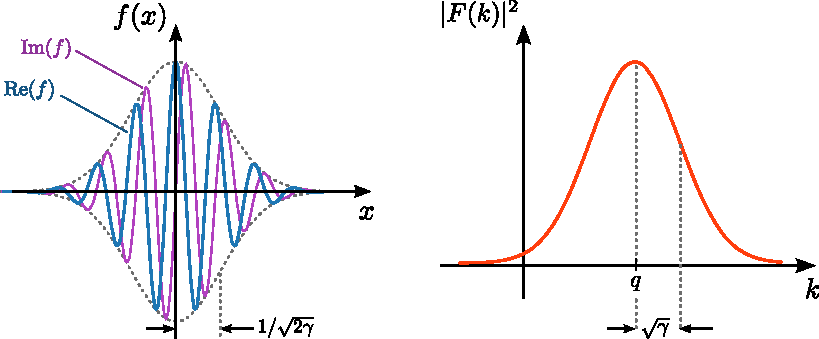
\includegraphics[width=0.65\textwidth]{fourier_example4}
\end{figure}
    
\subsection{The delta function}
\label{the-delta-function}

What happens when we feed the Fourier relations into one another?
Plugging the Fourier transform into the inverse Fourier transform, we
get
\begin{align}
  f(x) &= \int_{-\infty}^\infty \frac{dk}{2\pi} \, e^{ikx} F(k) \\
&= \int_{-\infty}^\infty \frac{dk}{2\pi} \, e^{ikx} \int_{-\infty}^\infty dx' e^{-ikx'} f(x')\\
&= \int_{-\infty}^\infty dx' \int_{-\infty}^\infty \frac{dk}{2\pi} \, e^{ikx}  e^{-ikx'} f(x')\\
  &= \int_{-\infty}^\infty  dx' \; \delta(x-x')\, f(x'),
\end{align}
In the last step, we have introduced
\begin{equation}
\delta(x-x') = \int_{-\infty}^\infty \frac{dk}{2\pi} \, e^{ik(x-x')},
\end{equation}
which is called the \textbf{delta function}. According to the above
equations, the delta function acts as a kind of filter: when we multiply
it by any function $f(x')$ and integrate over $x'$, the result is
the value of that function at a particular point $x$.

But here's a problem: the above integral definition of the delta
function is non-convergent; in particular, the integrand does not vanish
at $\pm \infty$. We can get around this by thinking of the delta
function as a limiting case of a convergent integral. Specifically,
let's take
\begin{equation}
\delta(x-x') = \lim_{\gamma \rightarrow 0} \, \int_{-\infty}^\infty \frac{dk}{2\pi} \, e^{ik(x-x')} \, e^{-\gamma k^2}.
\end{equation}
For $\gamma \rightarrow 0$, the ``regulator'' $\exp(-\gamma k^2)$
which we have inserted into the integrand goes to one, so that the
integrand goes back to what we had before; on the other hand, for
$\gamma > 0$ the regulator ensures that the integrand vanishes at the
end-points so that the integral is well-defined. But the expression on
the right is the Fourier transform of a Gaussian wavepacket
(Section~\ref{gaussian-wave-packets}). Using that result, we get
\begin{equation}
\delta(x-x') = \lim_{\gamma \rightarrow 0} \; \frac{1}{\sqrt{4\pi\gamma}} \, e^{-\frac{(x-x')^2}{4\gamma}}.
\end{equation}
This is a Gaussian function, of width $\sqrt{2\gamma}$ and area
$1$. Hence, the delta function can be regarded as the limit of a
Gaussian function as its width goes to zero while keeping the area
under the curve fixed at unity (which means the height of the peak
goes to infinity).

The most important feature of the delta function is it acts as a
``filter''. Whenever it shows up in an integral, it picks out the value
of the rest of the integrand evaluated where the delta function is
centered:
\begin{equation}
\int_{-\infty}^\infty  dx \; \delta(x-x_0)\, f(x) = f(x_0).
\end{equation}
Intuitively, we can understand this behavior from the above definition
of the delta function as the zero-width limit of a Gaussian. When we
multiply a function $f(x)$ with a narrow Gaussian centered at $x_0$,
the product will approach zero almost everywhere, because the Gaussian
goes to zero. The product is non-zero only in the vicinity of
$x = x_0$, where the Gaussian peaks. And because the area under the
delta function is unity, integrating that product over all $x$ simply
gives the value of the other function at the point $x_0$.

\begin{framed} \noindent
  \textit{Note}---In physics, the delta function is commonly used to
  represent the density distributions of \textbf{point particles}. For
  instance, the distribution of mass within an object can be
  represented by a mass density function. Assuming one-dimensional
  space for simplicity, we define the mass density $\rho(x)$ as the
  mass per unit length at position $x$. By this definition,
  \begin{equation*}
    M = \int_{-\infty}^\infty \rho(x)\, dx
  \end{equation*}
  is the total mass of the object. Now suppose the mass is distributed
  among $N$ point particles, which are located at distinct positions
  $x_1, x_2, \dots, x_N$, and have masses $m_1, m_2, \dots, m_N$.  To
  describe this situation, we can write the mass density function
  as
  \begin{equation*}
    \rho(x) = \sum_{j=1}^N \, m_j\, \delta(x-x_j).  
  \end{equation*}
  The reason for this is that if we integrate $\rho(x)$ around the
  vicinity of the $j$-th particle, the result is just the mass of that
  single particle, thanks to the features of the delta function:
  \begin{align*}
    \lim_{\varepsilon\rightarrow 0^+}\, \int_{x_j - \varepsilon}^{x_j + \varepsilon} \rho(x) \, dx &= \sum_{i=1}^N m_i\; \Big[\lim_{\varepsilon\rightarrow 0^+}\, \int_{x_j - \varepsilon}^{x_j + \varepsilon} \delta(x-x_i) \,dx\Big]\\ &= \sum_{i=1}^N m_i\; \delta_{ij} \\ &= m_j.
  \end{align*}
  Likewise, integrating $\rho(x)$ over all space gives the total mass
  $m_1 + m_2 + \cdots + m_N$.
\end{framed}

\subsection{Multi-dimensional Fourier transforms}
\label{multi-dimensional-fourier-transforms}

When studying problems such as wave propagation, we will often have to
deal with Fourier transforms acting on several variables simultaneously.
This is conceptually straightforward. For a function
$f(x_1, x_2, \dots, x_d)$ which depends on $d$ independent spatial
coordinates $x_1, x_2, \dots x_d$, we can Fourier transform each
coordinate individually:
\begin{equation}
F(k_1, k_2, \dots, k_d) = \int_{-\infty}^\infty dx_1\; e^{-ik_1x_1}\; \int_{-\infty}^\infty dx_2\; e^{-ik_2x_2}\,\cdots\, \int_{-\infty}^\infty dx_d\; e^{-ik_d x_d}\, f(x_1,x_2, \dots,x_N)
\end{equation}
Each coordinate gets Fourier-transformed into its own independent $k$
variable, so that the result is still a function of $d$ independent
variables.

We can express this kind of ``multi-dimensional Fourier transform'' more
compactly using vector notation. If $\vec{x}$ is a $d$-dimensional
coordinate vector, the Fourier-transformed coordinates can be written as
$\vec{k}$, and the Fourier transform is
\begin{equation}
F(\vec{k}) = \int d^d x \; e^{-i\,\vec{k}\,\cdot\,\vec{x}}\, f(\vec{x}),
\end{equation}
where $\int \int d^d x$ denotes an integral over the entire
$d$-dimensional space, and $\vec{k}\cdot\vec{x}$ is the usual dot
product of two vectors. The inverse Fourier transform is
\begin{equation}
f(\vec{x}) = \int \frac{d^dk}{(2\pi)^d}\; e^{i\,\vec{k}\,\cdot\,\vec{x}}\, F(\vec{k}).
\end{equation}
The delta function can also be defined in $d$-dimensional space, as
the Fourier transform of a plane wave:
\begin{equation}
\delta^d(\vec{x}-\vec{x}') = \int \frac{d^dk}{(2\pi)^d} \, e^{i\vec{k} \cdot \left(\vec{x}-\vec{x}'\right)}.
\end{equation}
Note that $\delta^d$ has the dimensions of $[x]^{-d}$. The
multi-dimensional delta function has a ``filtering'' property similar
to the one-dimensional delta function. For any $f(x_1,\dots,x_d)$,
\begin{equation}
\int d^dx \; \delta^d(\vec{x}-\vec{x}') \, f(\vec{x}) = f(\vec{x}').
\end{equation}


\subsection{Exercises}\label{exercises}

\begin{enumerate}
\item
Find the relationship between the coefficients $\{\alpha_n, \beta_m\}$
in the sine/cosine Fourier series and the coefficients $f_n$ in the
complex exponential Fourier
series:
\begin{align}
  f(t) &= \sum_{n=1}^\infty \alpha_n \sin\left(\frac{2\pi n x}{a}\right) + \sum_{m=0}^\infty \beta_m \cos\left(\frac{2 \pi m x}{a}\right) \\ &= \sum_{n=-\infty}^\infty f_n \exp\left(\frac{2\pi i n x}{a}\right).
\end{align}

\item
  Consider the triangular wave
  \begin{equation}
    f(x) = \left\{\begin{array}{rr}- x, &-a/2 \le x < 0, \\ x, & 0 \le x < a/2\end{array}\right.
  \end{equation}
  Derive the Fourier series expansion.

\item
Prove the properties of the Fourier transform listed in
Section~\ref{basic-properties-of-the-fourier-transform}.

\item
  Find the Fourier transform of $f(x) = \sin(\kappa x)/x.$

\item
  Prove that if $f(x)$ is a real function, then its Fourier transform
  satisfies $F(k) = F(-k)^*$.
\end{enumerate}
\end{document}
